\documentclass[12pt]{article}
\usepackage{xeCJK}  
\input{../common/common.tex}
\usepackage{indentfirst}


\setCJKmainfont[BoldFont = STSongti-SC-Bold]{STSongti-SC-Regular}
\ setCJKfamilyfont {here} {SIL-Hei-Med-Jian}% 宋体
\setCJKfamilyfont{song}{SimSun} %宋体
\ setCJKfamilyfont {kai} {Kaiti}% 楷体
\setCJKfamilyfont{fang}{song} %Imperial Song
\setCJKfamilyfont{li}{song} % Lishu
\setCJKfamilyfont{you}{Yuanti} %Yuanyuan

\newcommand{\song}{\CJKfamily{song}} %宋体
\newcommand{\hei}{\CJKfamily{hei}} %黑体
\ newcommand {\ kai} {\ CJKfamily {kai}}% 楷
\newcommand{\fs}{\CJKfamily{fang}} %Imperial Song
\newcommand{\li}{\CJKfamily{li}} % Lishu
\newcommand{\you}{\CJKfamily{you}}	%幼圆
\newcommand{\reffig}[1]{图\ref{#1}}
\newcommand{\refsec}[1]{\S \ref{#1}}

\onehalfspacing % ----------Set 1.5 times line spacing (may make sense, to be adjusted)

%\parindent=20pt % ------------------- The first line is indented, and the English segment is directly 0pt.
\setlength{\parindent}{2.1em}
\setlength{\parskip}{0.3\baselineskip}
\newcommand{\dom}{{\; \texttt{dom}\;}}
\newcommand{\xpcomment}[1]{{\color{blue} #1}}

\setCJKsansfont[BoldFont = STHeitiSC-Medium]{STHeitiSC-Light}


\newtheorem{property}{Features}
%\addbibresource{reference.bib}

\begin{document}
\pagestyle{empty}
\renewcommand{\contentsname}{catalog}
\renewcommand{\abstractname}{Abstract}
\renewcommand{\refname}{References}
%\renewcommand{\nomname}{Glossary (sorted by initials)}
\renewcommand{\figurename}{图}
\renewcommand{\tablename}{表}
\renewcommand{\baselinestretch}{1.5}
\renewcommand{\appendixname}{Appendix}
\renewcommand{\proofname}{proof}

%\pagecolor{\pcolor}

\begin{titlepage}
  \begin{center}
    \vspace*{5.5cm}
    \includegraphics[scale=0.4]{../common/Nebulas.png}
    \vspace{0.5cm}


    \textbf{\huge{Nebulas NAX White Paper}}

    \vspace{0.5cm}
    NextDAO Lab
    \ vfill
    August 2019\\
    Version number: 1.0.0
    \textbf{}
  \end{center}

\end{titlepage}
\setcounter{page}{0}
\tableofcontents
\newpage
\setcounter{page}{1}
\pagestyle{fancy}
\vspace*{0.01cm}
%% !TEX root = main.tex
\section{概述}

\textbf{关键字: Token Economy\ 经济体\ 去中心化\ 协作\ 激励\ 自进化\ 自治 }

\vspace{2em}

星云链(Nebulas)是开源公链,星云是\textbf{自治元网络}(Autonomous Metanet)~\cite{AutonomousMetanet},星云专注于处理复杂数据和交互、复杂的协作关系,致力于通过区块链等技术手段,实现让每个人从去中心化协作中公平获益的愿景~\cite{vision}。

NAX是质押币。

全新智能资产平台nextDAO致力于构建更好的去中心化自治组织,更好的Token经济(Better DAO, Better Token Economy),关注链上互动和协作,提供去中心化金融工具,重新定义Token经济,发现新的业务场景,推动生态应用落地。从星云生态起步,核心技术沉淀到星云链主网,鼓励从模式到范式的创新,最终形成通用模块,为更广泛的用户所用。
\section{星云理念概述}

\subsection{理念与愿景}
区块链技术本身不是一个全新的技术创新,而是作为一系列技术的组合(包括密码学,分布式系统,博弈论等)而产生的模式创新。比特币~\cite{Nakamoto2008}创造了“⼀个去中⼼化电⼦现⾦系统”的完美设计,从而打开了区块链世界的大门。以太坊~\cite{buterin2013ethereum}进一步提出了具有图灵完备性的代码的智能合约区块链框架,并发明了ERC20的范式,使得在区块链上融资变得更加便利。区块链技术也因此取得了空前的繁荣和发展。

在星云的白皮书~\cite{whitepaper}中也提出了自己的区块链理念,并持致力于践行“让每个人从去中心化的协作中公平受益”的愿景。同时也提出了自己的路径,其中包括:星云指数(NR), 开发者激励协议, 星云原力(NF)以及星云贡献证明(PoD)等。在过去两年中,星云链根据自身优势以及在区块链世界摸索前行的中总结的经验,将会有更多的探索和尝试。


\subsection{区块链协作}
随着科技的发展,协作场景已经从人与人面对面合作变得更灵活、更自由。区块链技术本质上是一个去中心化、非信任、基于博弈的自治体系,其真正的魅力是在去中心化思想下基于共识机制的开放协作模式。目前区块链的协作仍然存在着以下几个问题:

\begin{itemize}

	\item \textbf{协作角色多样化}

	早期比特币社区只有矿工和持币者,有了以太坊之后出现了开发者、应用使用者等,越来越多的人接触到区块链,不同用户角色的责权利如何分配受到挑战。

	\item \textbf{激励方式单一}

	目前大多数公链的共识激励还是以PoW, PoS为主的专注于挖矿的激励,事实说明单一激励不能应对用户角色的逐渐丰富。

	\item \textbf{公平与正向博弈缺失}

	为社区做出贡献的角色并没有得到对应的激励,使得整个区块链没有呈现出正向博弈的。

\end{itemize}
\section{The Better DAO}
什么是DAO? The DAO -- Decentralized Autonomous Organization,又叫“去中心化自治组织”。The DAO源于在以太坊上的股权融资技术,为组织规则以及决策机构编写代码,从而消除书面文件的需要,以及减少管理人员,从而创建出一个去中心化管理架构。2016年,以太坊The DAO被黑客攻击,并盗走价值千万美金的以太坊,最终导致以太坊硬分叉。虽然The DAO没有最终那么成功,但是这是一个伟大的尝试,并且也给了后续的工作带来了很多借鉴的作用。

\subsection{什么是Better DAO?}
以太坊ERC20的出现,成为了一种新的融资方式,以区块链智能合约技术为基础,资产发行的成本很低,在各种区块链代币交易平台支持下,代币发行后即可上市交易获得流动性,早期投资人退出时间大大缩短。但没有解决融资过后的问题,同时滋生了骗局。建立一个更完善的DAO体系,也是星云链技术发展的重要目标之一 -- 在去中心化的协作中公平受益,其实阐述的就是一个The Better DAO。

\subsection{A Better DAO - NAX}
如上所述,公链需要一个符合自身的Token Economy, 星云愿景是致于建立一个更好的协作平台,让参与者公平受益。公链建立自身的Token Economy常见、安全、系统漏洞低、防羊毛党的方式是Staking. 因此,星云将在NextDAO[x]框架下,提出一个以协作创新、激励贡献、刺激正向博弈、壮大社区共识、发展独有公链技术为目标的一个生态Token -- NAX。

在接下来的章节中会详细叙述NAX的核心逻辑以及可能的应用场景。
\section{The Design of the NAX}
\subsection{Design Goal}
In addition to forming a positive economic game and increasing ecosystem activity, the goals of the public chain token economics should also conform to certain principles such as fair benefits, positive incentives, logical simplicity while being capalbe of utilization in diverse scenarios. The public token economy requires fair access to scenarios and diverse consumption scenarios while retaining a high holding value thereby promoting the development and growth of the public chain making the entire ecosystem more dynamic. To sum up, the design goals of NAX include:

\begin{enumerate}[\hspace{2cm}(a)]
    \item fair benefits
    \item positive incentives
    \item simple and effective
    \item retains high utility
\end{enumerate}

\subsection{Core Mechanism}

\subsubsection{Equality Fairness}
The effectiveness of a public chain's token economy comes from the fairness and legitimacy of asset acquisition. The requirements for acquiring assets should be simple, transparent and an identical process for the vast majority of people. In the Nebulas economy, NAS assets owned by users are relatively fair and legitimate and due to this, the primary way to obtain additional tokens of a token is via Staking NAS. Equity token issuance must not be due to unclear requirements or loopholes existing which lead to the phenomenon of poor asset allocation. The overall result of token issurance must be conducive to improved ecosystem development on the public chain.

\subsubsection{Decentralized Staking - dStaking}
The traditional centralized staking method requires users to transfer assets into smart contracts for temporary custody. Asset security issues are maintained in a smart contract and unfortunately, smart contract asset security issues are common in the history of blockchain where hackers exploit contract loopholes and as a result the token holder suffer large economic loss. 

Due to this, pledging also puts great pressure on public chain project parties since a large number of assets are kept in a smart contract which makes them targets. Due to this, the management and security of smart contracts is a large development bottleneck. All assets on the blockchain are genuine and pledging simply locks in the liquidity of that asset - it does not validate the ownership of the asset (although it can be retrieved by calling the contract method) once transferred to the contract.

We propose a new mechanism of pledging: dStaking (decentralized Staking) as shown in the figure \ref{fig:dStaking}. This new method ensures the assets are still owned by the user; the user enters into a staking "contract" where the smart contract records the value of the staking. The purpose of a staking contract is simply to randomly verify whether the user is still fulfilling their contractual duties (e.g. pledging a minimum amount of NAS). When the balance of the pledging address is greater than or equal to the amount specified within the contract, it is considered a valid staking, otherwise it will be considered a canceled staking. The user is also able to add assets to their staking and the system recalculates an average age based on the new staking value which is discussed in the appendix.

The advantages of dStaking include:
\begin{enumerate}[\hspace{2cm}(a)]
    \item Protects user identification of assets
    \item Improve staking paritipation due to eliminated security risk
    \item Improve overall asset security
\end{enumerate}

\begin{figure}[htbp]
  \centering
  \includegraphics[width=1\textwidth]{../common/dStaking.pdf}
  \caption{Centralized staking vs decentralized staking\label{fig:dStaking}}
\end{figure}

\subsubsection{NAX Distribution Model - NDM}
As mentioned above, on the basis of safeguarding the equity and legitimacy of assets, and ensuring the inviolable ownership of staked assets, the user contributes the liquidity of their assets and in return, they obtain corresponding for participating in the ecosystem development. We call this new mode of token issuance "NDM" (Nebulas Devotional Mining). 

The maximum amount of NAX tokens that will be released is 10 billion(\(10^{10}\)) with an issuance cycle of every 6,000 blocks (approximately once per day tokens will be distributed). The number of tokens issued per cycle decreases with an attenuation coefficient of $\mu=0.999$ (reduction of 0.001\% every cycle) which leads to distribution completion in about 12 years. The number of pre-release NAX increases with the number of cycles, as shown in \ref{dist} and the cumulative number of pre-release NAXs is shown in \ref{acc}.

\begin{figure}[h]
\centering
\begin{minipage}[5cm]{.45\textwidth}
\centering
    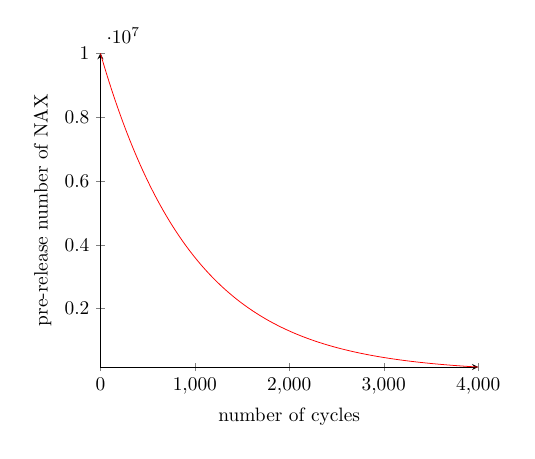
\begin{tikzpicture}[scale=0.7]
    \begin{axis}[
        axis lines = left,
        xlabel = {number of cycles},
        ylabel = {pre-release number of NAX},
    ]
    \addplot [
        domain=-0:4000, 
        samples=1000,
        color=red,
    ]
    {1.0*10^7*0.999^x};

    \end{axis}
    \end{tikzpicture}
\caption{Pre-release number and period relationship}\label{dist}

\vspace{\baselineskip}
\end{minipage}\qquad
\begin{minipage}[5cm]{.45\textwidth}
\centering
    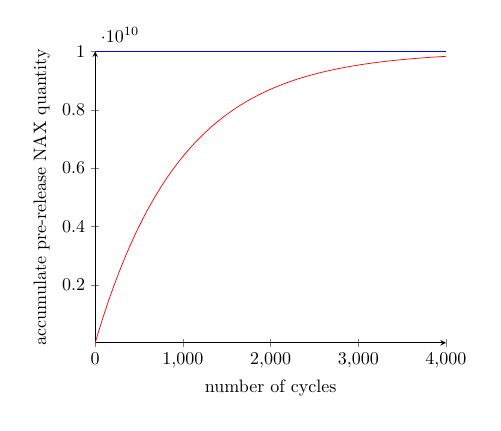
\begin{tikzpicture}[scale=0.65]
    \begin{axis}[
        axis lines = left,
        xlabel = {number of cycles},
        ylabel = {accumulate pre-release NAX quantity},
    ]
    \addplot [
        domain=-0:4000,
        samples=1000, 
        color=red,
    ]
    {10^10*(1 - 0.999^(x+1))};

    \addplot [
        domain=-0:4000, 
        samples=1000,
        color=blue,
    ]
    {10^10};
    \end{axis}
    \end{tikzpicture}
\caption{cumulative pre-release quantity and period relationship}\label{acc}
\end{minipage}
\end{figure}

\subsubsection{Dynamic Distribution Model}
The dynamic distribution model refers to fact that the system will determine the actual number of NAX to be distributed according to specific variables with the intention to promote a positive economic game. At the beginning of NAX, we will introduce the staking rate impact factor and dynamically adjusted the actual distribution ratio based on the increase or decrease of the staking rate. In the future, we will introduce more  factors as needed. As shown in the figure \ref{fig:dynamic_dist}, the system pre-distributes $C_i$ NAX to the users pledging in the current period within the period $i$. In the actual distribution process, according to the current staking rate level $\lambda$ (total amount of staking NAS/total NAS circulation, 0<$\lambda$<1), the actual distribution of NAX is: $C_0 \mu ^i\lambda$.

\begin{figure}[htbp]
  \centering
  \includegraphics[width=0.68\textwidth]{../common/dynamic_dist.pdf}
  \caption{Dynamic distribution strategy diagram\label{fig:dynamic_dist}}
\end{figure}

\subsubsection{Distribution cycle}
During a distribution cycle, different number of staking cycles will result in different distribution weights. The system determines the final NAX distribution amount based on the staking quantity of each staked user $V_{i, j}$ and the staking weight \(f(T_{i, j})\). If the $N$ address is being validly staked during the $i$ period, the $j$ address staking is $V_{i,j}$, and the effective staking period is $T_{i,j}$. Therefore, the number of NAXs that the address can be distributed to is $K_{i,j}$ as shown in the following formula.

\begin{equation}
  K_{i,j} = \frac{V_{i,j} f(T_{i,j})}{\sum_j V_{i,j} f(T_{i,j})} \lambda_i C_i
\end{equation}

Where \(f(T_{i,j})\) is the effective weight function for the staking of the \(i\) user\(j\). The relationship between the staking weight and the number of staking cycles is as follows (the function relationship is shown in figure \ref{weight}).
\begin{equation}
  f(T) = 1 - \frac{\sqrt{(aT+b)^2+c^2}-(aT+b)}{2}
\end{equation}

\begin{figure}[h]
\centering
    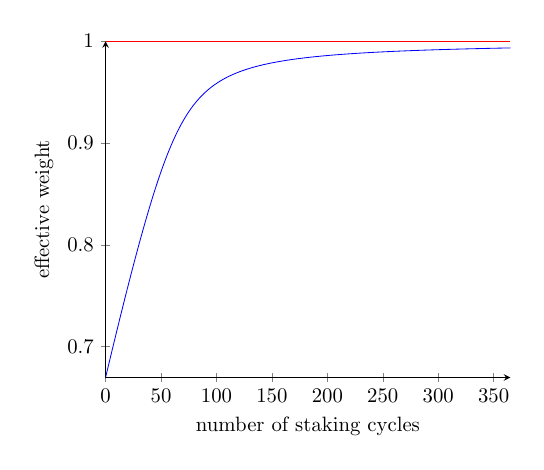
\begin{tikzpicture}[scale=0.75]
    \begin{axis}[
        axis lines = left,
        xlabel = {number of staking cycles},
        ylabel = {effective weight},
    ]
    \addplot [
        domain=0:365,
        samples=200,
        color=blue,
    ]
    {1-(sqrt((0.005*x-0.3)^2+0.2^2)-(0.005*x-0.3))/2};

    \addplot [
        domain=-0:365, 
        samples=200, 
        color=red,
    ]
    {1};
    \end{axis}
    \end{tikzpicture}
\caption{Relationship between the effective weight and the number of cycles}\label{weight}
\end{figure}

The parameters $a$, $b$, $c$, etc... in the formula are discussed in the appendix. In general, within the same cycle, the system allocates the total amount of additional issuance tokens according to the number of stakings and the corresponding length of the staking. In order to achieve a fair result, the more stakings and the longer the staking, the higher the issuance number will be. At the same time, this method increases the motivational levels of new staking users while motivating existing stakers since the existing addresses weight will be retained at a considerable level. The design will meet the following scenarios:

\begin{enumerate}[\hspace{1cm}(a)]
  \item Early users involved in staking have a greater probability of receiving more issuance.
  \item As the staking rate increases, the number of system issuance will increase accordingly to encourage more people to join the staking system.
\end{enumerate}

\subsubsection{NAX Ecosystem Fund Pool}
In order to facilitate economically better opportunities for development, incubation, support and other activities, a NAX eco-fund pool will be established. During the actual distribution process, the system will distribute it to staking users and deduct $5\%$ of the pool of funds held by the Nebulas Foundation are subject to community supervision. The specific content of the event will be disclosed after the publication of the white paper.

\subsection{Contract Framework}
NAX is an extensible NRC20 contract consisting of a set of contracts, data managment and parameters of the entire contract with multi-sign contracts, as shown in detail in \ref{fig:nax_framework}.

\begin{figure}[htbp]
  \centering
  \includegraphics[width=0.8\textwidth]{../common/nax.pdf}
  \caption{NAX contract component schematic \label{fig:nax_framework}}
\end{figure}

\section{NAX 应用场景展望}

各使用场景可以自行设定,奖励,销毁策略。

\subsection{Go Nebulas平台}

基金会资助Go Nebulas平台的300w NAS, 以及今后系统增发的部分NAS作为资助Go Nebulas平台经费,这些资金也将同时作为质押以获得NAX,作为社区贡献的附加奖励。

\subsubsection{分发场景}

星云社区化项目制的开放性平台,社区贡献者可以由分为几个角色:社区开发者,社区推广者。社区贡献者通过Go Nebulas上做项目,将会获得NAS的工资奖励, 同时将会获得额外的NAX的社区贡献奖励/凭证,根据项目的优先级,定义不同比例的NAX返比。

社区贡献者分类

\begin{enumerate}[a.]
  \item 项目开发
  \item 运营/PR
  \item 市场拓展
  \item 拉新
  \item 基础设施:
  \item 主网
\begin{enumerate}[i.]
  \item NAS nano Pro
  \item 硬件钱包
  \item 新钱包对接
  \item 跨链合作
\end{enumerate}
\end{enumerate}

为了鼓励社区贡献者的积极性,我们初步确定以下的返NAX比例参数:

普通项目 :S * x * N (NAS reward)

优先项目(基础设施):T * x * N (NAS reward)

(s < t)

\subsubsection{消耗场景}
\begin{enumerate}
\item 创建提案(消耗相应的NAX)
\item 开发提案(开发时会销毁等比的NAX, 提前完成的工作,节省销毁的数量)
\item 投票通过提案和结果,需要销毁后NAX(通过或以获得120\%返还,失败可以获得110\%的返还)
\end{enumerate}

推进步骤
\begin{enumerate}
\item 补发过去参与过贡献的人的奖励?
\item 以后获得项目资金的人将获得相应NAX奖励
\item 增加GN邀请奖励,受邀请的贡献者获得的NAX后,邀请人会获得额外10\%的NAX
\end{enumerate}

\subsection{星云治理 - 提升社区参与度}
为了鼓励社区使用NAX作为社区治理的工具,以及鼓励大家社区治理的参与度,我们将设置一些投票场景,部分场景投票将做会有返还奖励。
投票的场景

\subsubsection{节点竞选 -- PoD}
\begin{enumerate}[a.]
  \item 从节点候选人里可以选出节点
  \item 投票销毁后会返还(若当选,获得120\%返还,失败有110\%返还)
  \item 参与节点竞选, 需要销毁1000W NAX,具体参与需要再调整
  \item 成为节点, 被选中成为出块节点后,参与到节点出块,需要质押NAS(无NAX返还)
\end{enumerate}

\subsubsection{理事竞选}
\begin{enumerate}[a.]
  \item 从候选人里选出相应的理事
  \item 投票销毁后会返还(若当选,获得120\%返还,失败有110\%返还)
\end{enumerate}


\subsection{星云生态上币费}
NAS nano Pro \& Explorer \& DEX等各类生态平台的上币费/手续费
随着Next DAO的推进以及社区治理的前进,社区里将会出现越来越多的Token和治理尝试。这些币种都将需要相应的工具支持,所需要上NAS nano Pro和Explorer的需求。资源空间有限的情况下,我们可以采取增加上币费的需求,比如需要在NAS nano Pro和Explorer上币的NRC20需要缴纳 500w NAX(参数可调)的上币费。其中20\%归集给NAS nano Pro和Explorer管理团队 (开发者和运营者)80\%会被销毁

\subsection{社区预留NAS销毁计划}
与其将3500w NAS一次投票销毁,其实可以把销毁做成一项长期的社区投票活动,由社区来决定这个事情的发生。

销毁细节:

每个自然月1号发起一次投票销毁社区预留剩余NAS总量的 \(\alpha\) \% , \(\alpha\) \% 是当前NAS 质押率占流通量的份额。

投票销毁通过细节:

\begin{enumerate}[a.]
  \item 投票需要满足 \(\alpha\) \%的现行NAX总量,才合格
  \item 支持销毁的比例超出50\%
  \item 投票销毁,只返还50\%
\end{enumerate}

\section{总结}
星云为了更好地实现的理念与愿景,结合自身生态的特点,提出了适应自身理念和发展的通证经济。在整个文章当中,我们分析了NAX的公平性,正当性,确权性,激励性等,贯穿整个星云的理念、生态建设、发展、协作与治理。这只是我们开展NextDAO方向的一个示范和开端。在这个过程当中,更多有趣,有价值的想法将会涌现出来,同时期待社区的加入一起丰富NextDAO的内容。

% \ Printbibliography
\newpage
\bibliography{reference}

\newpage 
\begin{appendices}
\section{NAX分析}

\subsection{发行量分析}

略,以后添加

\subsection{反作弊分析}

略,以后添加


\section{Change Log}
\begin{itemize}
\item{0.0.1} Release. 2019.8
\item{0.0.2} Release. 2019.11 (Update some legal terms)
\end{itemize}

\end{appendices}
\end{document}
